\section{Requirements}

All building blocks in this thesis are developed with the purpose in mind to give the user the ability to visualize and interact with complex 2D and 3D data while being able to easily extend the library.
To enable this kind of functionality, a lot of parts of the infrastructure need to work seamlessly together.
Certain design choices had to be made to guarantee this. As speed is the most constraining factor, this chapter will start by introducing the design choices that were made in order to achieve state of the art speed.

\vspace{1em}
\begin{minipage}{\linewidth}
    \centering
    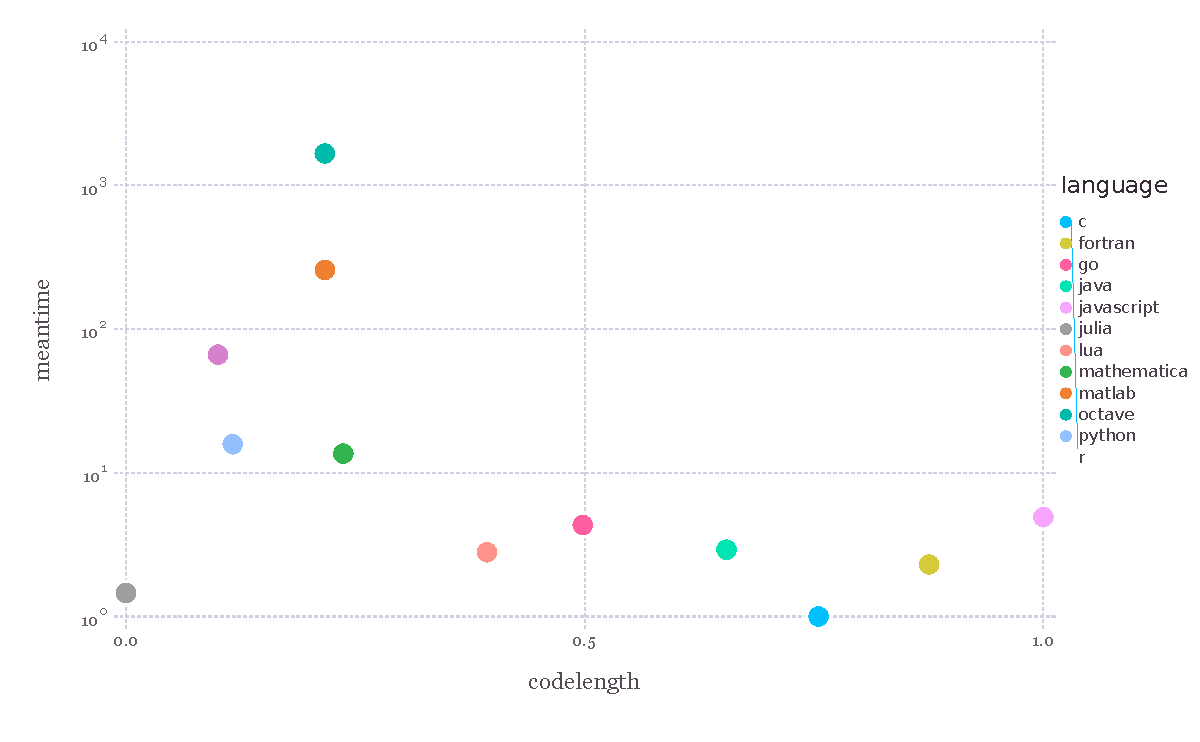
\includegraphics[width=0.9\linewidth]{graphics/julia_bench.pdf}
    \captionof{figure}[Volume Visualization]{Languages speed relative to C (averaged benchmark results), plotted against the length of the needed code (Source in Appendix).}
    \label{fig:juliabench}
\end{minipage}


\subsection{Speed}
Speed is mainly a usability factor. It is a factor that can make a software unusable, or render it unproductive. Because of this, speed has taken a high priority in this thesis. 
As general coding productivity is also a concern, this thesis is set on using a high-level language.
Historically, these two demands cannot be satisfied at the same time.
How to achieve state of the art speed with a high-level language is an ongoing research and basically the holy grail of language design. 
Julia promises to do exactly this, which is illustrated in Figure \cref{juliabench}. 
The code length is an ambiguous measure for conciseness, but if the code is similarly refactored and implements the same algorithm, it is a good indicator of how many lines of code are needed to achieve the same goal.
From this figure we can conclude, that Julia at least comes close to its promises. This is one of the reasons why it has been chosen as the programming language for this project.

There are a lot of libraries out there which can be used as a basis for implementing a 3D visualization library.
If you start to take the previous demands into account, the options shrink down considerably.
The visualization library should be implemented in one high-level language, which can be used for scientific computing and has state of the art speed. 
At this point, there are close to zero libraries left. As you can see in figure \cref{juliabench}, Matlab, Python, and R disqualify, as they are too slow. JavaScript, Java, Go, and Lua are missing a scientific background and the others are too low level for the described goals.
This leaves only Julia, but in Julia there were no 3D libraries available, which means that one has to start from scratch.
There are only a couple of GPU accelerated low-level libraries available, namely Khronos's \ac{OpenGL}, Microsoft's DirectX, Apple's Metal and AMD's Mantel, which are offering essentially the same functionality. 
Only \ac{OpenGL} is truly cross-platform, which is why \ac{OpenGL} has been chosen.
To access \ac{OpenGL} from within Julia a wrapper had to be written. 
This leaves us with one binary dependency not written in Julia, namely the video driver, which implements \ac{OpenGL}.

Measurement of success is pretty straightforward, but the devil is in the detail.
It is easy to benchmark the code, but quite difficult to find a baseline, as one either has to implement the whole software with an alternative technology or one has to find similar software.
This thesis will follow a hybrid strategy, comparing some simple implementations with different technologies and choose some rivaling state of the art libraries as a baseline.

\subsection{Extensibility}
Extensibility is an important factor in scientific computing, as a lot of flexibility is needed when exploring new horizons. 
It is not only that, but also a great factor determining the growth of a library. The more extensible the software is, the higher is the probability that someone else contributes to it.
In order to write extensible software, we first have to clarify what extensibility is.
Extensible foremost requires that the code is accessible. There are different levels of accessibility. 
The lowest level is closed source, where people purposely make the code inaccessible. While this is obvious, it is just a special case of not understanding the underlying language. 
Shipping binaries without open sourcing the code means that the source is only accessible in a language which is extremely hard to understand, namely the machine code of the binary. So another example for inaccessibility is to write in a language that is difficult to understand. 
Other barriers are obfuscated language constructs, difficult compilation procedures, missing documentation and cryptic highly optimized code.
Furthermore, the design of the library in the whole is an important factor for extensibility. It is not only important that all parts are understandable, but also that every independent unit in the code solves only one problem. 
This guarantees that one can quickly exchange it, or use it somewhere else where the same problem needs to be solved.
If this is guaranteed, re-usability in different contexts becomes much simpler. 
This allows for a broader user base, which in turn results in higher contributions and bug reports.
Short and concise code is also important, as it will take considerably less time to rewrite something, as the amount of code that has to be touched is shorter and less time is spent on understanding and rewriting the code.

The code written for this thesis will be open source, modular, written in a high-level language and concise.

This is pretty difficult to measure as these are either binary choices, which are followed or not or higher level concepts like writing concise code, which can be a matter of taste.
To get an idea of the effectiveness of the strategy, usage patterns and feedback from Github will be analyzed.

\subsection{Event System}
The event system is a crucial part of the library, as the proclaimed goal is to visualize dynamic, animated data.
This means, there are hard demands for usability and speed on the event system.
The chosen event system has an immediate influence on how to handle animations. 
The cleanest abstraction for animations and events are signals. Signals represent values that change over time.
If well implemented, it makes it natural to reason about time, without the need of managing unrelated structures and callback code.
Reactive\cite{Reactive} was chosen for this as it offers the nice abstraction of signals. It will be discussed in more detail in chapter \cref{reactive}.

\subsection{Interfaces}

Working with a computer means working with interfaces to a computer, which in the end simply juggles around with zeros and ones. There is a huge hierarchy of abstractions involved, to make this process of binary juggling manageable to the human.
The lowest relevant abstraction the programming language.
The next level of abstraction is the general architecture of the modular components, which has been discussed previously. 
This section specifies the \ac{API} design choices made.

The first \ac{API} is the \ac{OpenGL} layer. 
The chosen philosophy was to make the wrapper for native libraries as thin and reusable as possible and a one-to-one mapping of the underlying C-library.
This guarantees reusability for others, who want to work with the low-level library. Also, they might disagree with some higher-level abstractions and prefer to write their own.
The developed library is called ModernGL\cite{ModernGL}.

Over this sits an abstraction layer needed to simplify the work with \ac{OpenGL}, namely GLAbstraction\cite{GLAbstraction}.
Base on this abstraction, GLVisualize\cite{GLVisualize} was implemented, which renders the \ac{OpenGL} accelerated visualizations.

\ac{API}s for visualization libraries are very difficult to realize, as there are endless ways of visualizing the same data.
The design choice here was to use Julia's rich type system to better describe the data. 
Julia makes this possible, as one can create different types for the same data without losing performance.
One can create a type representing a unit like meters which has the same performance footprint as a native floating point type, but the visualization function can specialize to this with multiple-dispatch.
This way, a single function, e.g. \textit{visualize}, can create a default visualization for every different data types. 
Instead of manually passing additional information to the visualization function most information is already encoded into the type itself.
Together with the event system \cref{reactive}, it is possible to edit and visualize rich data with a simple interface. 
This is perfect for visual debugging, as it is always the same function call applied to the data. 
It makes it possible to visualize variables without further user interaction.
For a more fine grained control of the visualization more information is needed.

To pass addition information, key word arguments are used. An optional argument to the function is a style type, which controls the chosen defaults and the type of the visualization.
So for a float matrix, the default visualization may be a height-field, but passing the style \texttt{text} to the function might change the default to render a textual representation of the matrix.
This makes it easy to extend the visualize function, as the user just has to overload the function with a custom style together with optional key word arguments.
Finally, there are also graphical user interfaces developed for this thesis. As optimizing them is out of the scope of this thesis, they are kept very simple.
The measurement of success is again relatively difficult to evaluate.
Best would be to make a user poll to get actual feedback from people that use the software. This is a pretty demanding task, so instead the interface will just be evaluated analytically.


\section{Used Technologies}

\subsection{The Julia Programming Language}

The basic introduction to Julia has already been given in the Background chapter.
This chapter is focused on how to write programs with Julia and if it satisfies the requirements.
Most influential language construct are its hierarchical type system and multiple dispatch.
Multiple dispatch is in its core function overloading at runtime. 
To better understand multiple dispatch, one has to be familiar with Julia's type system.
The type system builds upon four basic types\cite{DBLP:journals/corr/BezansonEKS14}.
Composite types, which are comparable to C's structs and can be mutable or immutable, parametric composite types, bits types, abstract and parametric abstract types.
While the first three are all concrete types, abstract types cannot be instantiated but are used to build a type hierarchy.
Every concrete type can only inherit from one abstract type, while abstract types can also inherit from abstract types.
Bit types are just immutable, stack allocated memory chunks, usable for implementing numbers.
You can build type hierarchies like this:
\begin{lstlisting}
abstract Number
abstract FloatingPoint{Size} <: Number # inherit from Number
bitstype 32 Float32 <: FloatingPoint{32} # inherit from a parametric abstract type
type Complex{T} <: Number
    real::T
    img::T
end
\end{lstlisting}

With this type hierarchy one can overload functions with abstract, concrete or untyped arguments.

\begin{lstlisting}
foo{T}(y::Complex{T}, y::Float32) = println("some number: ", x, " some complex Number: ", y) # shorthand function definition
function foo(x)
    println("overloading foo with a new unspecific signature")
end
\end{lstlisting}

What will happen at runtime is, that Julia compiles a method specialized on the arguments which result in overloading the function with a method with concretely typed arguments.

In the case of \textit{foo}, it is initially overloaded with two methods.
Now, if one calls \textit{foo} with one \textit{Float32} argument, a new method will be added at run time, specialized to the\textit{Float32} argument.
Like this, if the function does not access non constant global values, all types inside the function will be known at call time.
This allows Julia to statically compile the function body, while propagating the type information down the call tree.

With multiple dispatch, Julia is more of a functional oriented language. 
But there are also ways to use Julia in a more object oriented style.
Functions are first-class, so they are easy to pass around. 
They can be bound to variables and can then be called like normal functions via the variable name. This implies that functions can also be bound to objects.
There is no self-reference available in Julia so the object still needs to be passed to the function via the arguments

Another crucial feature is the very simple, overhead free C interface. 
Thanks to the binary compatibility of \ac{LLVM}'s emitted assembly, a C function call to a shared library inside Julia has the same overhead as it would be from inside C\cite{CCALL}. 
This is perfect for integrating low-level libraries like \ac{OpenGL} and \ac{OpenCL}.

Julia's performance is crucial for this thesis. 
If Julia does not perform close to C it would weaken the whole argument of writing the visualization library in Julia.
This is why a performance analysis is done to prove that Julia is a good choice for a high performance visualization library.

It is a very tedious task to write representative benchmarks for a programming language. 
The only way out is to rely on a multitude of sources and try to find analytical arguments.
In this thesis, Julia's own benchmark suite will be used in addition to some real world benchmarks.
In addition, the general compiler structure of Julia will be analyzed to find indicators for the limits of Julia's performance.

\vspace{1em}
\begin{minipage}{\linewidth}
    \centering
    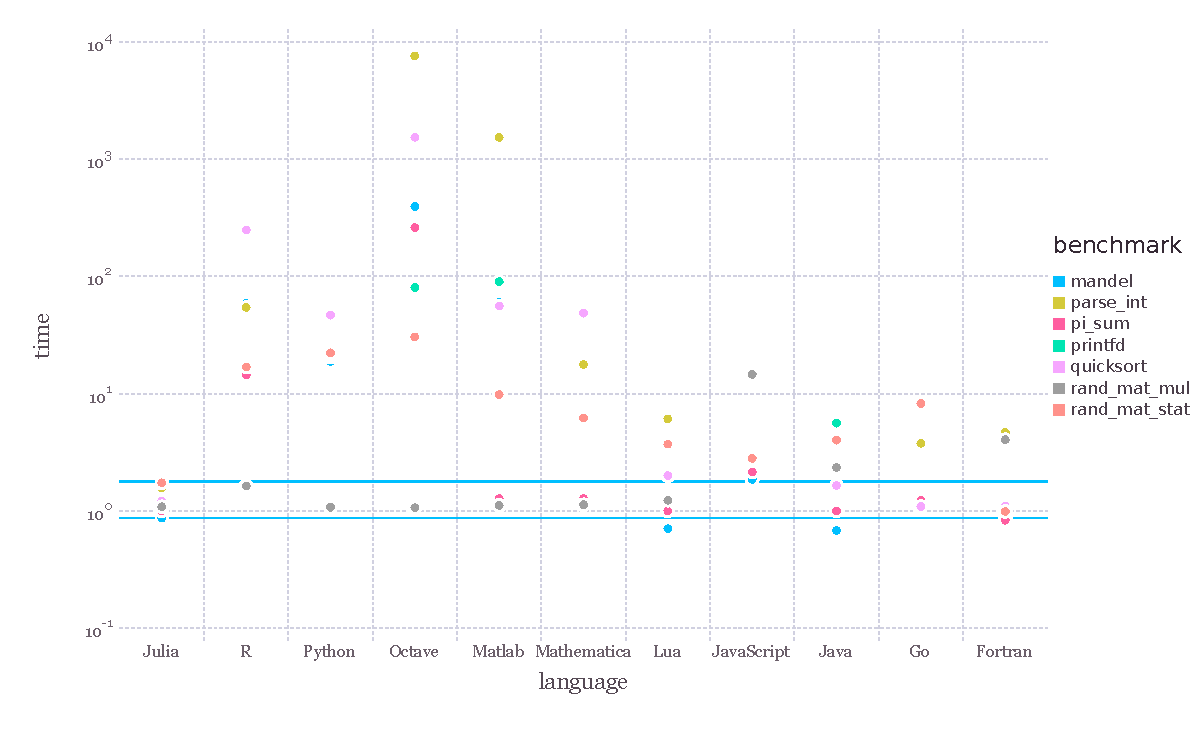
\includegraphics[width=0.9\linewidth]{graphics/juliabench.pdf}
    \captionof{figure}[Julia Performance]{Julia's performance compared to other languages, taken from Julia's micro bench suite \cite{JuliaBench}. Smaller is better, C performance = 1.0.}
    \label{fig:juliabench}
\end{minipage}

In the first benchmark from figure \cref{juliabench}, we can see that Julia stays well within the range of C speed. 
Actually, it even comes second to C-speed with no other language being that close.
This is a very promising first look at Julia, but it should be noted, that these benchmarks are written by the Julia core team and the performance of a language is a moving target.
So it is not guaranteed, that there is no bias favoring Julia in these benchmarks.
Another benchmark was found, which compares C++, Julia and F\#. It was created by Palladium Consulting\cite{PalladiumConsulting} which should not have any interest in favoring any of the languages.
They compare the performance of C++, Julia and F\# for an IBM/370 floating point to IEEE floating point conversion algorithm.
The results\cite{JuliaFSCpp} have been, that F\# comes out last with 748.275 ms, than Julia with 483.769 ms and finally C++ with 463.474 ms. 
At the citation time, the Author had updated the C++ version to achieve 388.668 ms. 
It looks like the author was only working on making the C++ version faster, so it cannot be said that the other versions could not have been made faster too.

The last Julia benchmark is more real world oriented. 
It is comparing Finite Element solver, which is an often used algorithm in material research and therefore represents a relevant use case for Julia.

\begin{table}[htbp]
    \centering
    \begin{tabular}{l|c|c|c}
        \hline
        \textbf{N}  & \textbf{Julia} & \textbf{FEniCS(Python + C++)}  & \textbf{FreeFem++(C++)}\\
        \hline
        121         & 0.99           & 0.67             & 0.01 \\
        2601        & 1.07           & 0.76             & 0.05 \\
        10201       & 1.37           & 1.00             & 0.23 \\
        40401       & 2.63           & 2.09             & 1.05 \\
        123201      & 6.29           & 5.88             & 4.03 \\
        251001      & 12.28          & 12.16            & 9.09 \\
        \hline
    \end{tabular}
    \captionof{table}[FEM Benchmark]{Performance of a FEM solver written in Julia compared to some existing libraries. \cite{FMSolver}}
    \label{table:fembench}
\end{table}
These are remarkable results, considering that the author states it was not a big effort to achieve this. After all, the other libraries are established FEM solvers written in C++, which should not be easy to compete with.

This list could go on, but it is more constructive to find out Julia's limits analytically.
As already mentioned, Julia is statically compiled at runtime. This means, as long as all types can be inferred at runtime, Julia will have in the most cases identical performance to C++.
The biggest remaining difference in this case is the garbage collection. 
Julia 0.3 has a mark and sweep garbage collector, while Julia 0.4 has an incremental garbage collector.
As seen in the benchmarks, it does not necessarily introduce big slowdowns.
But there are issues, where garbage collection introduces a significant slowdown\cite{ReadDlmGC}.
Analyzing this further is not in the scope of this thesis, though. 
But it can be said that Julia's garbage collector is very young and only the future will tell how big the actual differences will be.
Another big difference is between different compiler technologies.
Julia uses \ac{LLVM}\cite{Lattner:MSThesis02} for compilation.
In order to further understand Julia's potential, a further look at \ac{LLVM} is taken in the next section.

\subsubsection{\ac{LLVM}}

\ac{LLVM} is a compiler infrastructure, which has front ends for different languages and compiles to different platforms like x86, ARM, \ac{OpenCL} (SPIR) and \ac{CUDA} (NVPTX). 
A language designer must create an \ac{AST} which \ac{LLVM} can convert into \ac{LLVM} \ac{IR}. This \ac{IR} forms a standardized basis for any optimization step. Every language that can be converted to \ac{LLVM} \ac{IR} can be combined at this level. \ac{LLVM} itself offers many optimizations, but also third party optimization can be integrated.
This yields superior language interfacing for \ac{LLVM} based languages, as inlining and other optimizations can be done over the boundary of one language.
This is why Julia can look forward to having one of the best C++ \ac{FFI}\cite{Cxx}.

\ac{LLVM}'s concept is effective, as it makes it possible to accumulate state of the art optimizations in one place, making them accessible to many languages. Because of the many back-ends, languages that use \ac{LLVM} can run on many architectures. While Julia does not support all back-ends yet support will be added in the future.
\ac{LLVM} is also used by Clang\cite{Clang}, the C/C++ front end for \ac{LLVM} rivaling \ac{gcc}\ac{gcc}, it is used by Apple's programming language Swift\cite{SWIFT} and for Mozilla's language Rust\cite{Rust}.
This makes \ac{LLVM} a solid basis for a programming language, as these are highly successful projects guaranteeing \ac{LLVM} further prospering.
To see where \ac{LLVM} stands considering performance, one can compare it with \ac{gcc}, which is one of the most successful open source compilers for C++.
If C++ code that is compiled with \ac{gcc} is much faster than the same code compiled with \ac{LLVM}, the \ac{gcc} version will also be faster than a comparable Julia program.
In order to investigate the impact of this, a benchmark series written by Phoronix will be analyzed.
They benchmarked \ac{gcc} 4.92 against \ac{LLVM} 3.5 and \ac{LLVM} 3.5 against \ac{LLVM} 3.6.
Here is a summary of their exhaustive benchmarks:
\begin{table}[ht]
  \centering
  \begin{tabular}{l|c|c}
    \hline
    \textbf{Statistic} & \textbf{\ac{gcc} vs \ac{LLVM} 3.5} & \textbf{\ac{LLVM} 3.5 vs \ac{LLVM} 3.6} \\
    \hline
    mean & 0.99 & 0.99 \\
    median & 0.97 & 1.00 \\
    maximum & 1.48 & 1.10 \\
    minimum & 0.39 & 0.88 \\
    \hline
  \end{tabular}
    \captionof{table}[gcc vs llvm summary]{Summary of the Phoronix benchmark. Unit is speedup of \ac{LLVM}, bigger is better. \cite{LLVM35vsLLVM36}\cite{LLVMvsGCC}\cite{Phoronix}}
    \label{table:gccvsllvm}
\end{table}

The full tables can be found in the appendix under the table \cref{llvm35vsllvm36} and \cref{llvmvsgcc}.
The results suggest, that \ac{LLVM} is well in the range of \ac{gcc}, even though that there can be big differences between the two.
These are promising results, especially if one considers that \ac{LLVM} is much younger than \ac{gcc}. 
With big companies like Apple\cite{GoogleAppleLLVM}, Google\cite{GoogleAppleLLVM}, Mozilla\cite{Rust}, AMD\cite{LLVMAMD}, NVidia\cite{LLVMNvidia} and Microsoft\cite{MicrosoftLLVM} being invested in LLVM, it is to be expected that \ac{LLVM} will stay competitive, which means Julia should in theory stay competitive as well.


\subsection{\ac{OpenGL}}

\vspace{1em}
\begin{minipage}{\linewidth}
    \centering
    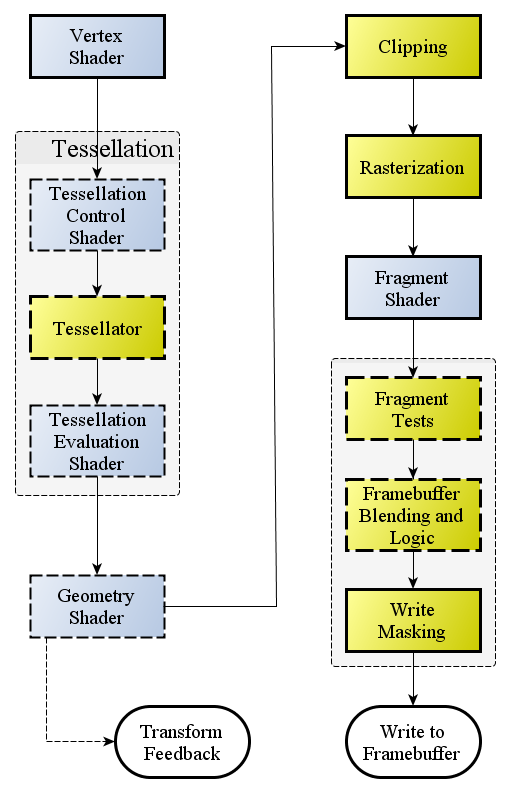
\includegraphics[width=0.5\linewidth]{graphics/RenderingPipeline.png}
    \captionof{figure}[OpenGL]{Diagram of the Rendering Pipeline. The blue boxes are programmable shader stages. Arrows show the flow of data\cite{OpenGLPipeline}}
    \label{fig:opengl}
\end{minipage}



\ac{OpenGL} is a low-level graphics API worked out by the Khronos Group\cite{Khronos} and implemented by the video card vendor via the video driver. 
As such it does not offer much abstraction over the actual \ac{GPU}, but instead offers high flexibility and performance.
\ac{OpenGL} 1.0 was released in 1992 and the current version is 4.5.
A critical element when developing \ac{OpenGL} applications is, that not all video drivers implement the newest \ac{OpenGL} standards.
As a result, one has to decide which \ac{OpenGL} version to target, trading between modernity and platform support.
For Romeo, it was decided to support \ac{OpenGL} 3.1 as the lowest bound, as it is sufficiently available, while still having most of the modern features.
All features that help to call less OpenGL functions can be considered as modern, as they take away the load from the CPU.
The modern features used in this thesis include instance rendering, vertex arrays and shader programs written in \ac{GLSL}.

In Figure \cref{opengl} the basic architecture of an OpenGL program pipeline is shown.
As the description states, the blue boxes are programmable shaders, while the dotted boxes are optional parts of the pipeline.
The yellow boxes describe stages which are not directly accessible. They are part of the global OpenGL state, which can be set via OpenGL commands.

So in order to have a working OpenGL rendering pipeline at least a vertex shader and a fragment shader needs to be written.
All shaders are compiled and linked into a program object, which can be executed on the \ac{GPU}.
Shaders are written in \ac{GLSL}, which is a C dialect specialized for vector operations.
You feed shaders with data via buffers, textures and uniforms. Buffers are 1D arrays, textures 1D/2D/3D arrays with both having their own memory, while uniforms live in the program object.

The different shaders are usually used to apply geometric and perspective transformations and calculating the light.
In newer APIs general compute operations are available, making it possible to create more flexible shader stages.
Displaying objects can only be achieved by rasterizing pixels to the frame buffer via the fragment shader.
The frame buffer can be sent directly to the monitor.
Frame buffers can contain multiple render targets, which are the buffers the fragment shader can write to.
The write operation is heavily restricted. The fragment shader can only write to the location calculated by the vertex shader and simultaneously reads from the frame-buffer are not possible. 
This restriction exists to allow for the massive parallel execution model that OpenGL uses to speed up rendering times.

The usual set of render targets includes a depth channel, stencil buffer and of course the color buffer.
The depth channel is usually used to discard all fragments that are behind another fragment (known as depth test), while the stencil buffer can be used to discard arbitrary fragments based on the stencil mask. 
Custom render targets can be created in newer OpenGL versions which can be written to via the fragment shader.
Here is a simple minimal example for a program rendering some vertex data with a flat color to the screen.

\begin{lstlisting}
//Vertex Shader
in vec3 vertex; // vertex fed into the shader via a buffer
uniform mat4 projection; // Projection matrix
uniform mat4 view; // View matrix, setting rotation and translation of the camera
void main()
{
    gl_position = projection*view*vec4(vertex, 1); // apply transformations to vertex and output to fragment shader
}
//Fragment shader
out vec4 framebuffer_color; //color render target, which will get written to the display
void main()
{
    framebuffer_color = vec4(1,0,0,1); // write a red pixel at gl_position from the vertex shader.
}
\end{lstlisting}

All visualization code is written in OpenGL shaders, which are compiled and executed via GLAbstraction.

\subsection{Reactive}\label{reactive}
Reactive\cite{Reactive} is a functional event system designed for event driven programming.
It implements Elm's\cite{Elm} signal based event system in Julia.
Signals can be transformed via arbitrary functions which in turn create a new signal.
This simple principle leads to a surprisingly simple yet effective way of programming event based applications.

\begin{lstlisting}
a = Input(40)       # an integer signal.
b = Input(2)        # an integer signal.
c = lift(+, a,b)    # creates a new signal with the callback plus. Equal to c = a+b
lift(println, c)    # executes println, every time that c is updated. 
push!(a, 20)        # updates a, resulting in c being 22
#prints: 22
push!(b, 5)         # updates b, resulting in c being 25
#prints: 25
\end{lstlisting}

Lifting a signal creates a callback, which gets called whenever the signal changes.
There are more operations than lifting, like folding, merging, filtering and so on.
With this, one can build up a complex tree of operators which will get applied to the original signal.
For the concrete case of Reactive, every signal carries around a list of children and parents.
Each signal has a rank, in order to build up a sorted heap with these information.
So every time a signal is updated, the heap can be traversed and the functions get applied in the right order, updating all the values of the children.
Reactive is used in all parts of the library. It builds the basis for the camera code, the widgets and any value that needs to be animated is realized via a signal.

\subsection{GLFW}
GLFW\cite{GLFW} is a cross platform \ac{OpenGL} context and window creation library written in C.
GLFW allows to register callbacks for a multitude of events like keyboard, mouse and window events.
Every operating system exposes this functionality in a slightly different way, making it very hard to create a window and to retrieve window events.
So a library like GLFW is crucial if one does not want to waste a lot of time just to implement all the corner cases for all the different operating systems out there.
In addition, GLFW exposes low level features like the operating systems \ac{OpenGL} context handle.
This can be used for creating advanced contexts that share memory with another context.
Romeo does not use this feature yet, but it makes GLFW a future proof choice.


\section{Implementation}

\vspace{1em}
\begin{minipage}{\linewidth}
    \centering
    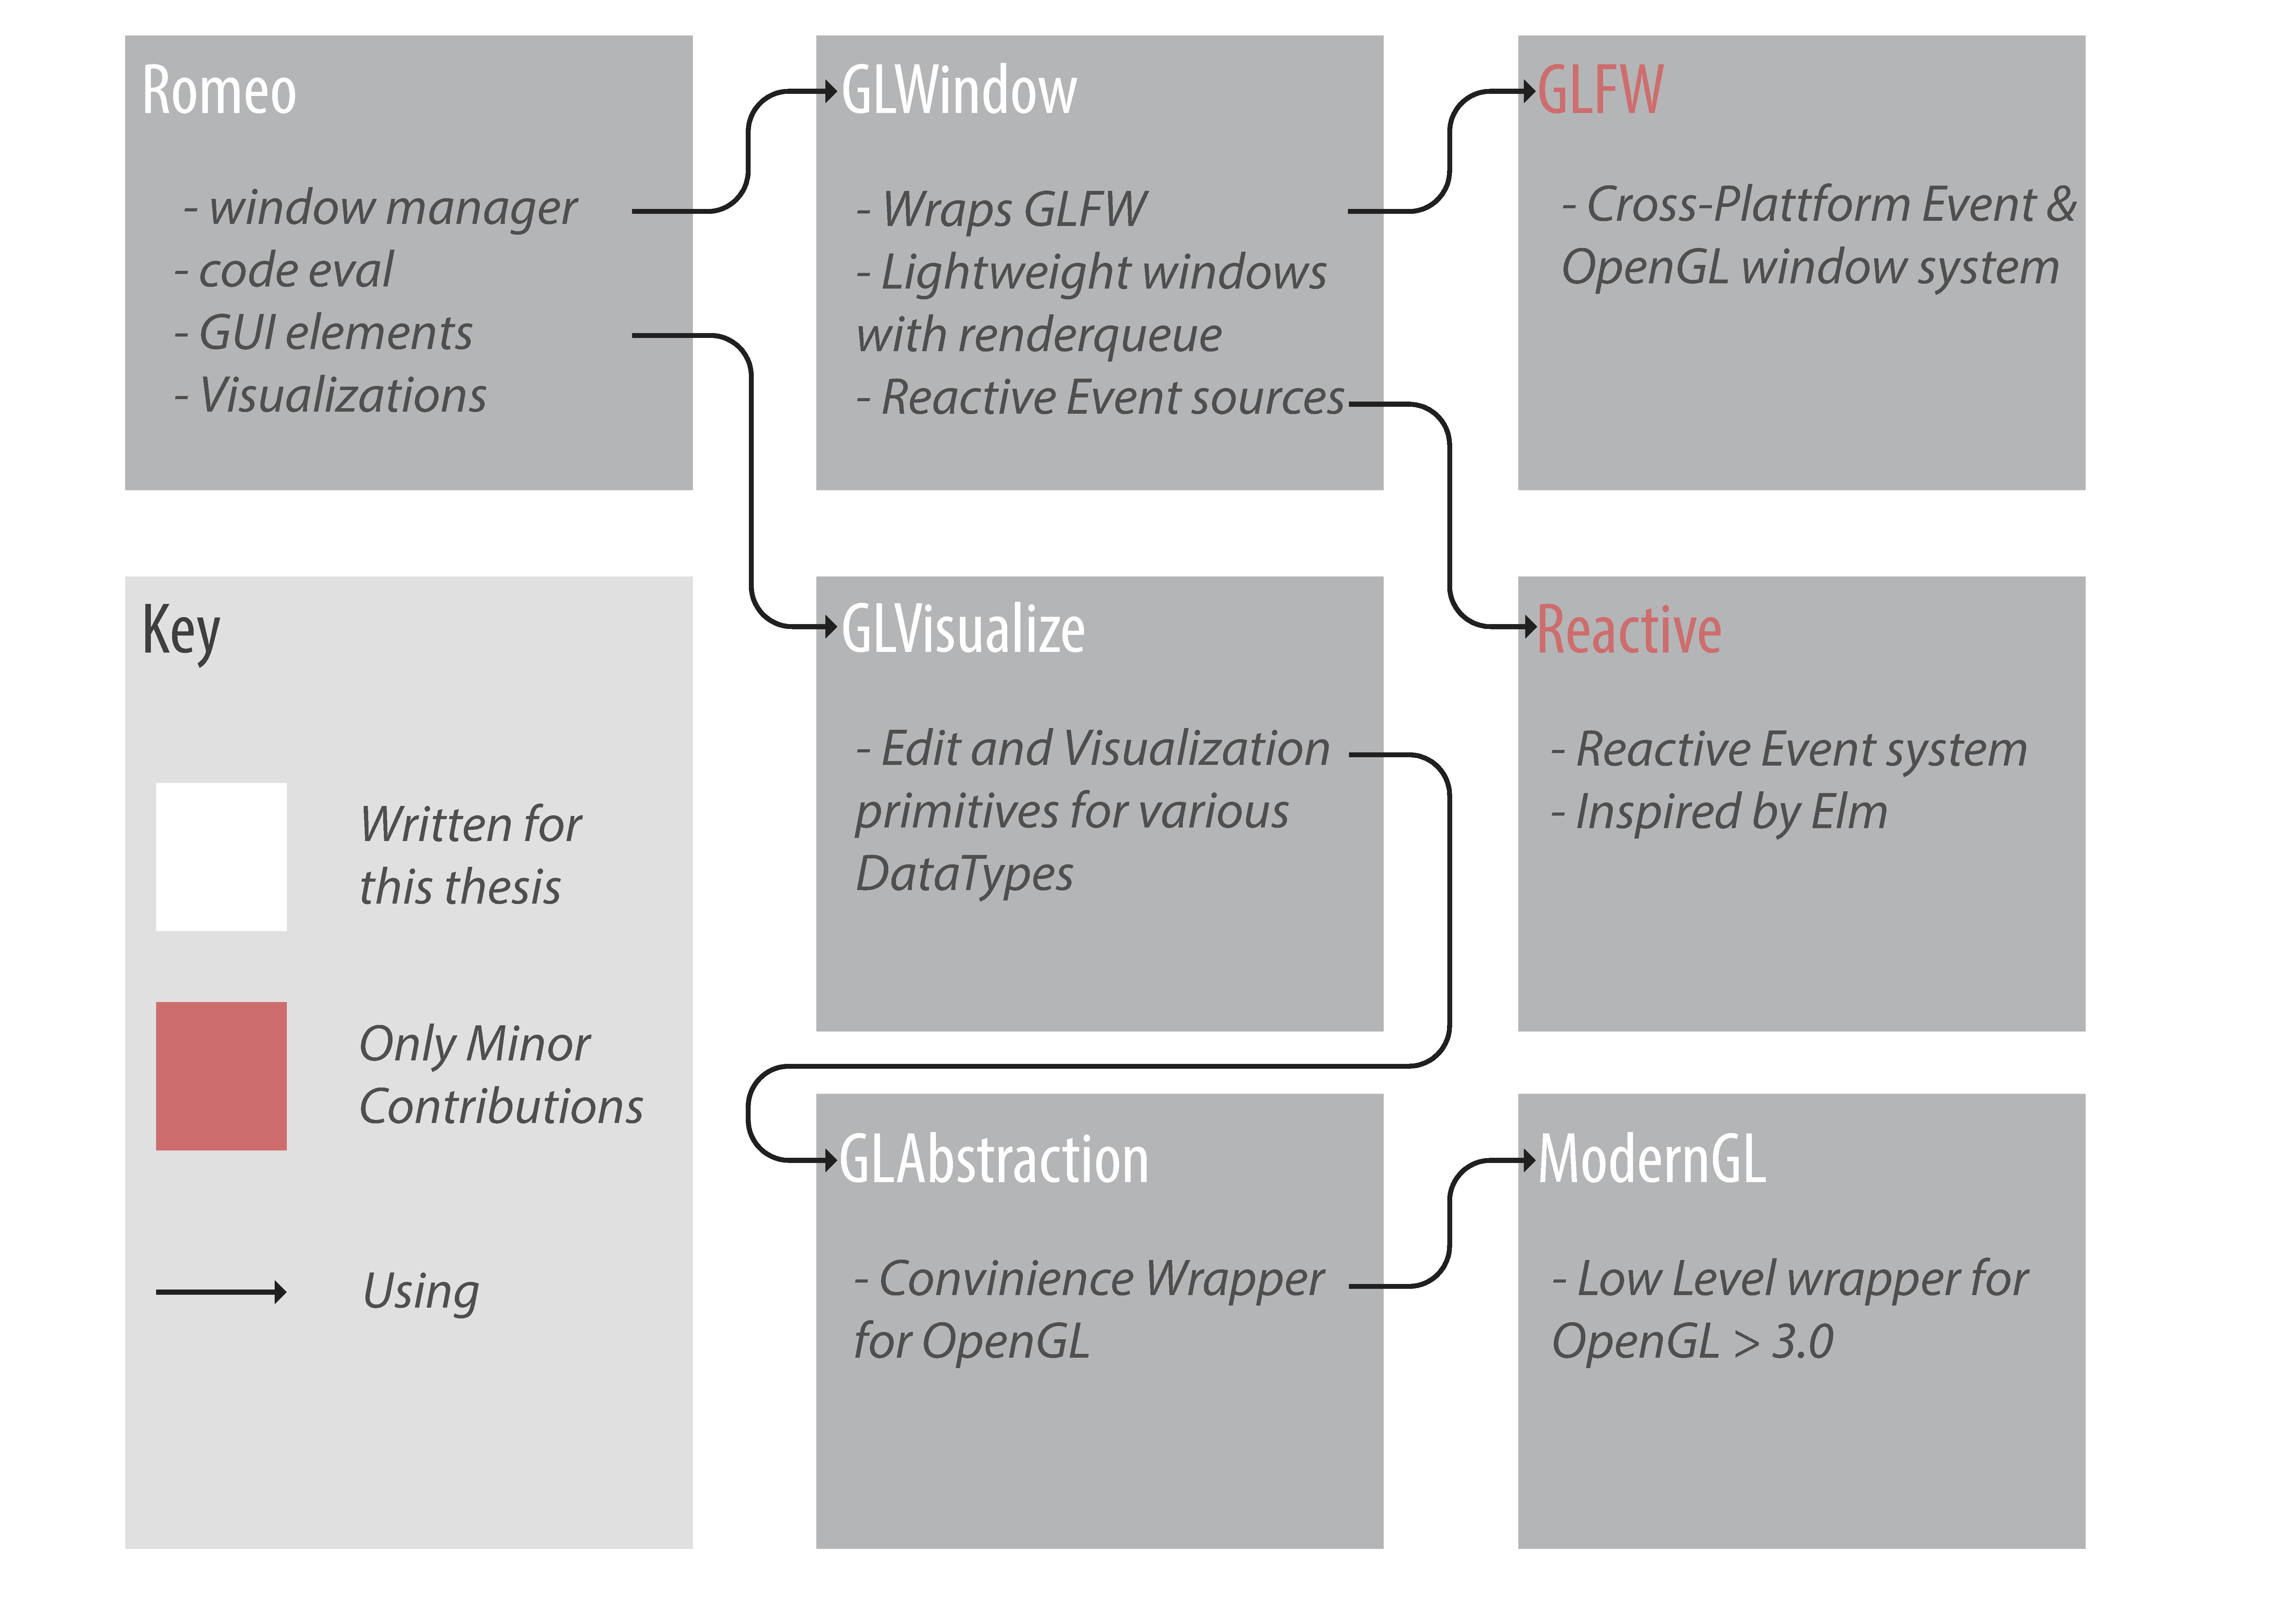
\includegraphics[width=0.9\linewidth]{graphics/architecture.pdf}
    \captionof{figure}[Architecture]{Main modules used in Romeo and their relation (simplified).}
    \label{fig:architecture} 
\end{minipage}


This chapter is about the implementation of Romeo and GLVisualize.
The Romeo package itself is small and just defines the high-level functionality of the editor.
This includes window layout and connecting all the different event sources to create the desired behavior.
Romeo relies on a multitude of packages, which step for step abstract away the underlying low-level code that is used for the window creation and rendering. 
As already pointed out in the requirements, special care has been taken to make all modules self-sufficient. 
Every single package can be used for other applications, which allows for higher flexibility and a broader user base.
ModernGL can be used by any OpenGL project which strives to build a low-level OpenGL program.
GLWindow and GLAbstraction can be used to build slightly higher level OpenGL visualizations. 
GLVisualize can be used to build other interactive visualization packages besides Romeo.

As shown in Figure \cref{architecture}, Romeo uses GLVisualize for creating \ac{GUI} elements and the visualizations. Romeo's code evaluation is done via Julia built-in functions and text fields are created with GLVisualize.
Windows are managed by GLWindow. 
GLWindow creates an OpenGL window with the help of GLFW and converts all window events into Reactive's signals. 
It also offers a very simple render queue, for rendering graphics attached to a window.
Signals are not only used as the event sources, but are also the main abstraction for time varying values in GLVisualize.
GLVisualize is the main package offering the rendering functionality and the editor widgets like text fields and sliders.
For rendering, GLVisualize relies on GLAbstraction, which defines a high-level interface for ModernGL.
ModernGL implements the \ac{OpenGL} function loading and exposes all the function and Enums definitions from \ac{OpenGL} with version higher than 3.0.



\subsection{ModernGL}
\ac{OpenGL} is implemented by the video card vendor and is shipped via the video driver, which comes in the form of a C library.
The challenge is to load the function pointers system and vendor independent. 
Also one further complication is, that depending on the platform, function pointer are only available after an \ac{OpenGL} context was created and may only be valid for this context. \cite{wgl}
This problem is solved by initializing a function pointer cache with null and as soon as the function is called the first time the real pointer gets loaded.

The OpenGL function loader of ModernGL has undergone some changes over time.
Starting with a very simple solution, there have been pull requests to improve it.
The current approach in ModernGL master was not written by myself, but by the Github user aaalexandrov\cite{Aaalexandrov}.
Before aaalexandrov’s approach, the fastest approach would have used a pretty new Julia feature, named generated functions.
It should in principle yield the best performance as it compiles a specialized version of the function when it gets called for the first time. This is perfect for \ac{OpenGL} function loading. When the generated function gets called the pointer can be queried and gets inlined into the just in time compiled function.

Generated functions only work with the newest Julia build, which is why aaalexandrov’s approach was favored.


\subsection{GLAbstraction}
GLAbstraction is the abstraction layer over ModernGL.
It wraps \ac{OpenGL} primitives like Buffers and Textures in Julia objects and hooks them up to Julia's garbage collector. 
It also makes it easy to create them from Julia data types like arrays and images.
Additionally, it implements convenience functions to load shader code and to provide the shader with the correct data types.
Besides supplying an abstraction layer over \ac{OpenGL}, it also offers the linear algebra needed for the various 3D transformation and camera code.
Building upon that, it defines a signal based perspective and orthographic camera.

Signals are an important part of the infrastructure not only for the camera, but for everything that changes.
As an example, the function that creates an \ac{OpenGL} program also takes signals of shader source code. 
With every source code update the \ac{OpenGL} program gets recompiled, making it possible to interactively develop \ac{OpenGL} shader. The signal can come from file updates, or from some text editing widget inside Julia.

One of the main data types is the \textit{RenderObject}.
It combines uniforms, \ac{OpenGL} buffers, textures and programs. 
One can call \textit{render(::RenderObject)}, which executes the program with the given uniforms and buffers loaded into the program. 
Creating visualizations with GLAbstraction turns into writing the shader and then combining it with the needed data in form of OpenGL types.
When the program includes a fragment stage, calling \textit{render} results in the object being displayed on the screen. But it is also possible to use compute shaders as \textit{RenderObjects}, which then just write into the supplied buffers without displaying anything.

A lot of OpenGL functions are bothersome to use from within Julia, as the output has to be pre-allocated and gets then passed to the function.
These functions have been overloaded in GLAbstraction to return the value instead.
With only ModernGL the code would typically look like this:
\begin{lstlisting}
result = Ref{GLint}(-1) #using Julia's reference type
glGetShaderiv(shaderID, GL_COMPILE_STATUS, result)
result = result[] # dereferencing
\end{lstlisting}
With GLAbstraction this becomes possible:
\begin{lstlisting}
result = glGetShaderiv(shaderID, GL_COMPILE_STATUS)
\end{lstlisting}

Similarly, OpenGL does not overload functions, which means that a function that does the same for different types has a base name combined with different suffixes to indicate the type.
The function with the most methods is \textit{glUniform}, which has around 34 functions for all the different uniform types. 
It is used to set the value of an \ac{OpenGL} program uniform.
With GLAbstraction, \textit{glUniform} has been overloaded for all different types, including arrays and signals. So one can simply call \textit{glUniform} on the type without the need of looking up the correct suffix.
This has been achieved with a combination of overloading and generated functions.
The generated function puts together the right function name and inlines it into the \textit{glUniform} method specialized to the argument type.

A lot more of these simplifications have been done in order to leverage the usage of OpenGL with Julia.
This guarantees that the code in GLVisualize is very short and concise, making it easy to extend and maintain.

\subsection{GLWindow}
GLWindow is a lightweight wrapper around GLFW.
It mainly offers a screen type, which contains signals for all the different GLFW events. 
It also offers a hierarchical structure for nesting screens.
All the screen areas are signals, which makes it easy to change the screen area. 
This makes it simple to implement windows that react to changing the size of the windows or resized objects.


\subsection{Event System}

The event system was challenging to integrate for several reasons.
First of all Reactive is a functional event system, while \ac{OpenGL} relies heavily on global states, which are two perpendicular concepts.
Also, Reactive does not allow rearranging the event tree. 
One cannot create sub trees in advance and then fuse them together at run time.
This led to the design choice, that signals are sampled from a render loop.
This is sub-optimal approach, as sampling artifacts can occur, and frames are rendered even if the scene does not change.
In the future it will be desirable to work around this and bring the elegant functional approach from Reactive to OpenGL.


\subsection{GLVisualize}

\vspace{1em}
\begin{minipage}{\linewidth}
    \centering
    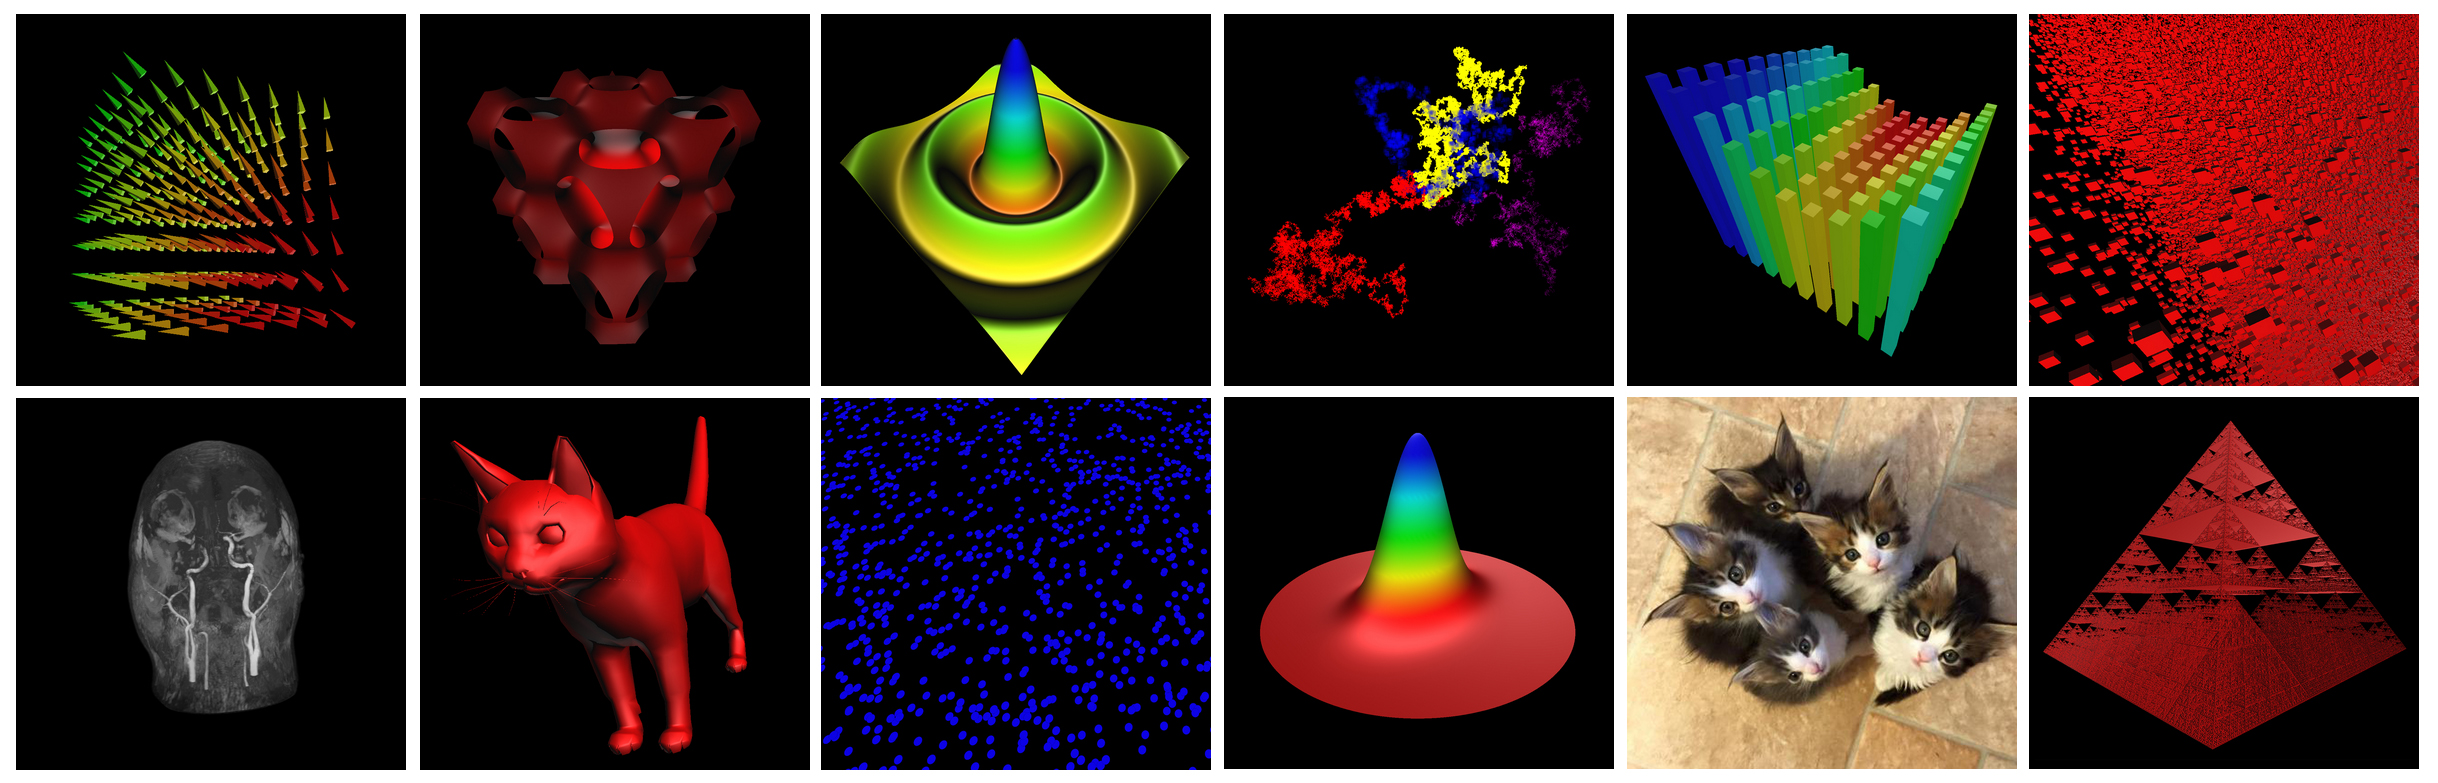
\includegraphics[width=0.9\linewidth]{graphics/glvisualize.jpg}
    \captionof{figure}[Visualisations]{Different visualizations rendered with GLVisualize.}
    \label{fig:glvisualize}
\end{minipage}

GLVisualize implements the visulization functionality.
Its structure is quite simple. 
It relies as much as it can on common Julia data types and creates specialized visualizations for them via dispatch.
So instead of offering differently named functions for different visualizations, there is just one function with lots of methods for different types, which is made possible via multiple-dispatch.
This has two advantages.
First, it makes it very easy to use for visual debugging, as any value can be displayed immediately without any user interaction.
Secondly, the user does not have to remember or lookup the function name, as long as there is a default visualization for the type he is working with.
The next design goal was to make this fit for dynamic data, which resulted in relying on as little transformation of the data as possible and directly transferring the data to the GPU.
Depending on the complexity of the visualization, this means the visualization can be updated with as little overhead as possible.

The interface to create visualizations is very simple and only consists of three functions:
\begin{lstlisting}
Dict{Symbol, Any}     = visualization_defaults(data::Union(Signal{T}, T), style::Style) # returns a dictionary of default parameters
RenderObject          = visualize(data::Union(Signal{T}, T), style=Style{:default}; parameters...) # returns an object which can be directly rendered
RenderObject, Signal  = edit(data::Union(Signal{T}, T), style=Style{:default}; parameters...) # returns an RenderObject and signal which outputs the changed values
\end{lstlisting}

With this simple interface, the following data can be visualized:

\begin{itemize}
    \item Text (Vector of Glyphs)
    \item Height fields with different primitives (Matrix of height values)
    \item 3D bar plots (Matrix of height values)
    \item Images (Matrix of color values)
    \item Videos (Vector of Images)
    \item Volumes (3D Array of intensities)
    \item Particles (Vector of Points)
    \item Vector Fields (3D array of directional Vectors)
    \item Colors (Single Color values)
\end{itemize}

All of these can be integrated into the same scene and it is possible to change their parameters interactively by passing signals.
These interactions can be purely programmatically, or via the widgets from the edit function.
The visualize methods that take Julia objects are transforming them into GPU objects, which will then get transferred to the actual visualize function. This function takes GPU objects as its arguments, making it easy to visualize objects which already exist on the GPU, or which are shared between visualizations.

Up to now, there is an edit function available for strings, colors, numbers, vectors and matrices.


\subsubsection{Mesh primitive Rendering}

The rendering of meshes in OpenGL is pretty straight forward with a normal vertex and fragment stage.
Vertex, Normal and UV data is supplied via Vertex Arrays and the perspective transformations via uniform matrices.
In the fragment shader, a Blinn-Phong lighting model is applied.

\subsubsection{Particle Rendering}

Most of the visualizations in GLVisualize are realized via instancing a mesh primitive.
So the bar plot is nothing else than a cube placed in a grid, with scaling information that get applied to every individual cube. The surface plot is a quad or any other 2D mesh spaced across a grid, while the vertexes are projected onto a height field. The vector field is a mesh placed on a 3D grid inside a cube, while the rotations from the direction vector gets applied to each individual mesh. 
Even text rendering functions in the same way. The difference is just, that the particle not only holds position information, but also indexes into a texture atlas in which renderings of the glyphs are cached. So when rendering the text particles, the exact scale and image of the glyph is queried, which will then be used to render a quad with the image of the particular glyph to the screen.
The texture atlas approach was chosen, because rendering a high quality vector graphic is very time consuming, especially if the description of the font is only available as a Bézier spline. A more detailed description can be found in chapter \cref{vector rendering}.
All particles are rendered via \ac{OpenGL}'s instanced rendering API, which allows to render millions of particles with only one draw call and very little memory usage, as the geometry of the particle just needs to be uploaded one time.
For every individual particle, additional information like color, position, scale and so forth can be queried from within the fragment or vertex shader stage.
This additional information can be stored in uniform buffers, uniform arrays or textures. Textures and texture buffers have been chosen for this thesis, as they offer the greatest support among devices and are easy to use. In the future, other approaches can be implemented, gaining more performance or flexibility.


\subsubsection{Vector Graphics Rendering}\label{vector rendering}
\vspace{1em}
\begin{minipage}{\linewidth}
    \centering
    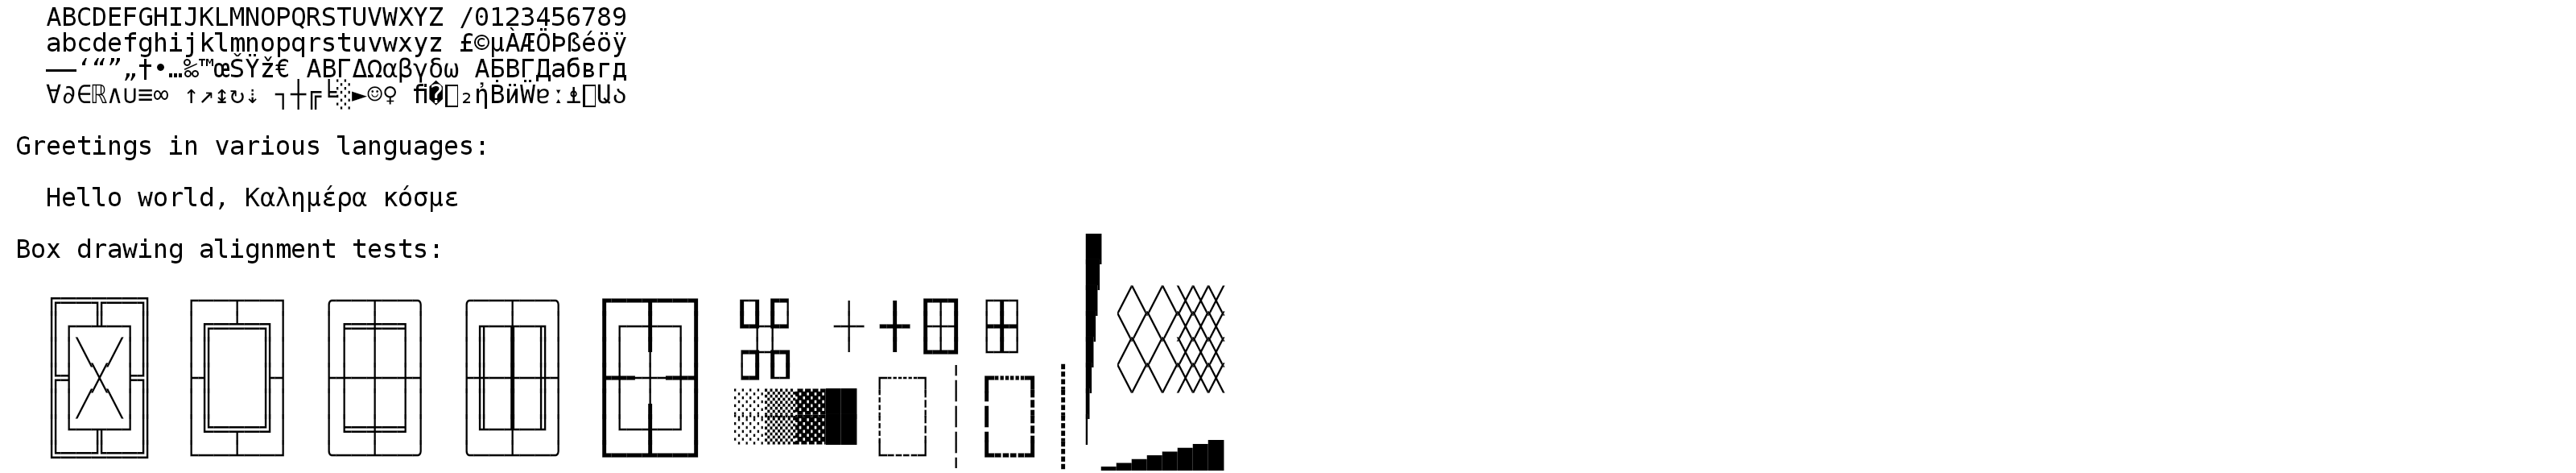
\includegraphics[width=0.9\linewidth]{graphics/utf8.png}
    \captionof{figure}[UTF8]{GLVisualize's fast UTF8 rendering with the help of FreeType, a texture atlas and 2D particles.}
    \label{fig:UTF8}
\end{minipage}

Vector graphics are difficult to render, as they are not a good fit for the \ac{GPU}.
Long stretched, curved and thin lines introduce several problems for the GPU\cite{Liland565821}.
Another problem is that splines used in vector graphics are usually supplied as Bézier curves, which are very demanding to rasterize.
Besides from that, anti-aliasing of thin lines introduces problems. 
With post processing anti-aliasing techniques, lines which are thinner than one pixel will introduce artifacts, as OpenGL primitives smaller than a pixel will get discarded by the \ac{OpenGL} pipeline. So additional care needs to be taken in order to assure, that primitives are always thicker than one pixel, or multi-sampling techniques have to be used.
This is only a very short summary of the problems, which is only given to illustrate that this is not a problem that can be solved in the scope of this thesis. 
Instead, FreeType\cite{FreeType} is used for rendering fonts. As FreeType is relatively slow, these renderings get cached in a texture atlas from which they can get queried and rendered to the screen in large numbers.
This results in high quality and fast renderings. This comes at the cost of higher space requirements and resolution dependence.
So when zooming into the vector graphics, either a new version has to be rendered or one gets pixelated results.
In the future, distance fields can be used to reduce the resolution dependence\cite{Green:2007:IAM:1281500.1281665}.

\subsubsection{Volume Rendering}
\vspace{1em}
\begin{minipage}{\linewidth}
    \centering
    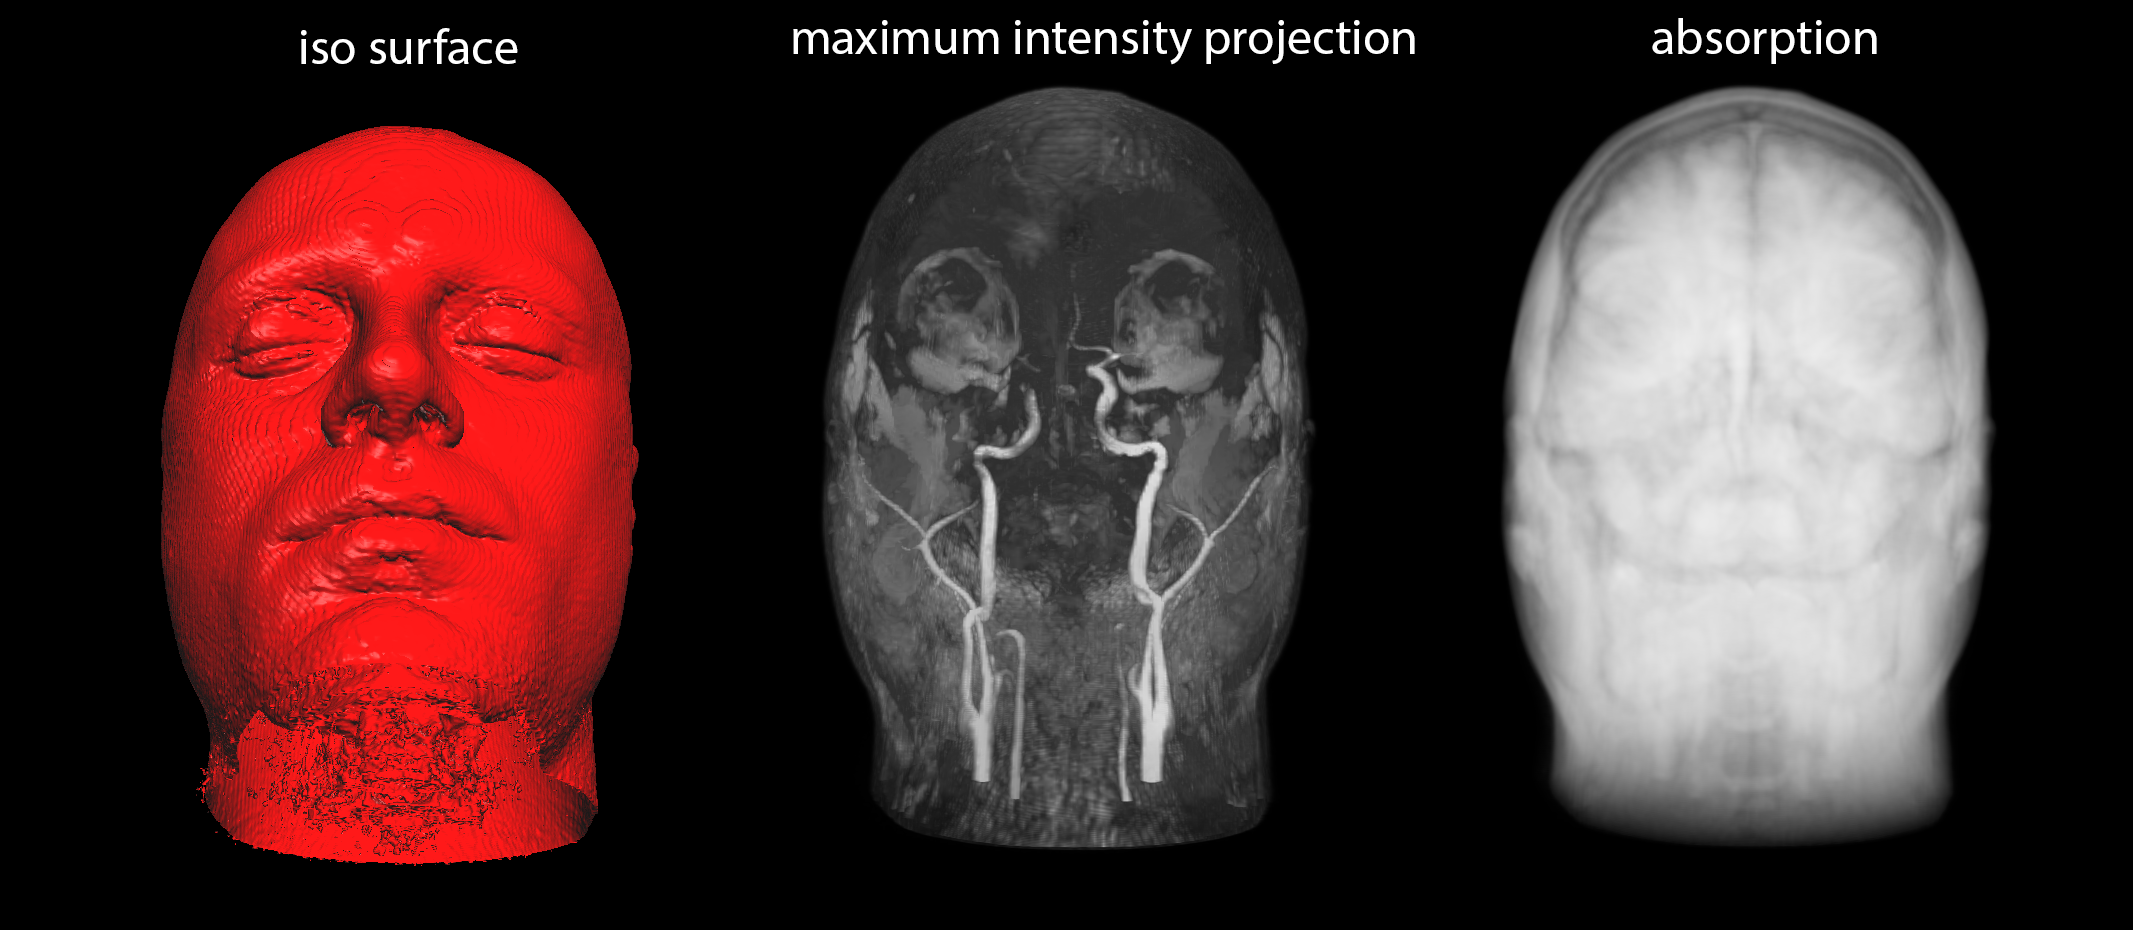
\includegraphics[width=0.9\linewidth]{graphics/volumes.png}
    \captionof{figure}[Volumes]{Different visualizations rendered with GLVisualize. As can be seen, every methods misses critical features of the volume.}
    \label{fig:volumes}
\end{minipage}

Volumes in 3D computer graphics are usually represented as voxels, which can be understood as 3D pixels. 
They represent values on a 3D grid. The name stems from the marriage of volume and pixel.
There are sparse and dense storage options for voxels and different information can be represented, like speed, rotation, color, intensities and so forth.
Volume renderings is not a trivial task. 
Not only from a computational point of view, but it is also difficult to make a visualization which shows the inside of a volume without hiding the surface. This is illustrated in figure \cref{volumes}.
This is why different forms of visualizations and interactivity are needed to get a good representation of a volume.
GLVisualize is able to render iso-surfaces, maximum intensity projections and an absorption based visualization form. 
On top of this, the particle systems can be used to give further insights into the volume by rendering particles for each voxel. This is especially helpful for sparse volumes.

For the Volume rendering two techniques are being used. 
Marching tetrahedra and ray casting\cite{marques2009gpu}. 
Marching tetrahedra is an algorithm that can be used to extract a mesh representation of an iso-surface from a volume.
Ray marching is the process of shooting rays from the camera origin through the object.
With every step inside the volume, values are sampled and depending on the combination of these values, different visualization forms can be realized. 
When stopped at a certain value, iso-surfaces can be rendered. 
If only the maximum is kept, it will yield a maximum intensity projection. 
When all values are combined via an absorption function, the volume will be displayed as if it is made of some translucent material like smoke.

The ray casting rendering method was explicitly implemented for this thesis on the GPU. For the marching tetrahedra algorithm there was already a Julia implementation available in the package Meshes.jl\cite{Tedrahedra}. The resulting mesh can be displayed with GLVisualizes mesh rendering capabilities.
Both techniques have their advantages and disadvantages. 
While marching tetrahedra is relatively slow, it can be used to generate a mesh which is very fast to display. 
Ray casting on the other hands allows for a wide range of visualization forms and is fast enough to calculate it for every frame. The downside is, that the calculation cannot be cached camera position independent. But it allows to interactively change the iso-values and all the other parameters, making it ideal to explore a volume.
 

\subsection{Scene Graph}
The scene graph is not a specialized data structure, but rather a list of objects, which can be directly rendered with OpenGL. Functionality from Reactive, GLAbstraction, GLVisualize and GLWindow are involved in this. GLVisualize creates a renderable object with GLAbstraction, which will get pushed into a render queue in the screen from GLWindow. Everything that moves is handled via signals from Reactive.
Asynchronously updating the signals and iterating over the render object list is achieved with Julia's simple asynchronous API. It is not truly multi-threaded, but rather creates a producer-consumer structure. It could be multithreaded, but this is more difficult to implement as \ac{OpenGL} is not thread safe.
This is an extremely simple form of a scene graph, which does not allow to perform any optimizations.
Optimizations usually include sorting in order to reduce OpenGL state changes and culling of invisible objects.
As GLVisualize produces OpenGL code which relies on very few calls to OpenGL, the first optimization is currently not as important.
But culling can make a large difference for big 3D scenes, as usually only a fraction needs to be rendered.
As this is a more involved process, which would preferably be done completely on the GPU, this was not in the scope of this thesis.

\subsection{3D Picking}

3D picking is the process of selecting a 3D object from a 2D projection like it is the case when one selects a 3D object on the screen with the mouse.
It forms the basis for any mouse interaction with objects displayed on the screen.
The two most usual approaches are ray picking and color picking.
For the ray picking approach a ray is send from the 2D position of the camera plane into the 3D scene and is tested for intersection with every object in the scene. In contrast, color picking works with an extra render target, which stores an object id for every pixel, which gets written together with the color pass inside the fragment shader.
Color picking has been chosen for this thesis, as it is far easier to implement. Ray picking must be implemented on the GPU, best with some data structures optimized to do fast ray intersections. Otherwise it will be very slow. If done on the CPU, the 3D objects need to be kept in video memory and CPU memory, further introducing complexity and bottlenecks.

For color picking, two frame-buffer render targets need to be created. 
One for the color channel and one to represent the object id plus an additional number to store contextual information. The additional number is usually used for the instance index, which can be used to e.g. infer what text glyph is selected.
When rendering, the fragment shader does not only write the color into the render target, but if the color is opaque also the current object id.
This way transparency aware 3D picking can be achieved without an extra processing step. 
The advantage of this methods is that one does not need an extra pass over the geometry. The disadvantage is higher space requirements and that OpenGL's native anti-aliasing does not work well together with the additional render target. Also, the OpenGL pipeline has to be flushed in order to read from the frame-buffer.
The anti-aliasing problem can be solved by implementing an extra anti-aliasing post processing step. A very simple FXAA algorithm has been implemented, which does not give perfect results but is fast and was easy to implement. The algorithm was taken from Matt DesLauriers\cite{FXAA} and was adjusted to fit into GLVisualize's pipeline.


\subsection{Romeo}

So far Romeo just consists of one file with 500 lines of code. 
It just defines some simple text field, a search field, and a visualize and edit window.
The texts gets evaluated as Julia code as soon as it changes. Like this, the text field acts like a very simple \ac{REPL}.
Via the search field, one can execute simple Julia statements and the results will be displayed in the visualize window, while all parameters can be edited via the edit window.
This means, if one types in a simple variable, the variable will be visualized. But one can also search and transform a variable via simple Julia terms.
In figure \cref{screenshot} a screens shot of Romeo can be seen.
On the left is a window for editing scripts. The middle is used to visualize bound variables, in this case the variable \textit{barplot} is visualized.
On the bottom of the middle, the variables can be selected via a text field. The text field allows to execute code, so one can do things like filtering an array which then will display the filtered array.
On the right all variables of the visualization can be edited interactively.
If one clicks on the color circle for example, a color chooser will pop up which will let one chose the color.
The numbers are sliders, so when one clicks and drags them, the value can be adjusted. 
While changing the values, the changes will be immediately displayed.

